\section{Bil} \label{sec:bil}

\subsection{DistanceSensor}
%%%%%%%%%%%%%%%%%%%%%%%%%%%%%%%%%%%%%%%%%%%%%%%%%%%%%%%%%%%%%%%%%
%																%
%      ++++++++++++ Design af Afstandssensor ++++++++++++++		%
%																%
%%%%%%%%%%%%%%%%%%%%%%%%%%%%%%%%%%%%%%%%%%%%%%%%%%%%%%%%%%%%%%%%%

Afstandssensorene leveres formonteret på chip hvor benene fra IC'en er trukket til harwinpins som let kan tilgås. Der benyttes I2C-protokol til kommunikation med Pi'en. Ved kommunikation benyttes følgende pins: 

\begin{itemize}
	\item pin 1: Temporary Default
	\item pin 2: Address Announce / Status
	\item pin 3: Benyttes ikke
	\item pin 4: SDA: Data
	\item pin 5: SCL: Clock
	\item pin 6: GND: Reference
	\item pin 7: VCC: Forsyning
\end{itemize}

\noindent
\textit{SDA}-linjen kommunikerer data ud med reference til GND.
\noindent
\textit{SCL}-linjen sørger for at holde timing. 
\noindent
\textit{AA/Status} benyttes til at angive om sensoren er i gang med at foretage en range- reading. Status-pin'en holdes højt så længe sensoren scanner, og trækkes lavt når operationen er fuldført. Dette angiver at data er klar til levering. Når status-pin'en er høj ignoreres al I2C-kommunikation, således at sensoren kan arbejde uforstyrret. 
\noindent
\textit{Temp-adresse}-pin'en benyttes til at initiere sensoren med en ønsket adresse, denne pin sætte høj ved power-up, kan en brugerdefineret adresse sendes til sensoren, i dette tilfælde benyttes unikke 8-bit adresser til sensorerne.

Herefter skrives en klasse \texttt{distanceSensor} der kan håndtere de ønskede kald til de 4 afstandssensorer. 
Denne klasse skal indeholde funktion til at tilgå sensorerne. Klassen initieres med constructoren hvori der åbne for I2C-devicet, samt at der sætte den foromtalte adresse. Detudover skal klassen indeholde metoden: \texttt{getDistance()}, i denne funktion foretages et read-kald med den pågældende sensors adresse. 
Følgende kommander benyttes for at kommunikere med en med en given adresse: 











\clearpage

\subsection{Klassediagram}
I dette afsnit beskrives det overordnede design på den software der kommer til at ligge på Pi. På figur \ref{fig:cd_pi} ses et klassediagram der opdeler funktionaliteten i klasser.

\begin{figure}[h]
\centering
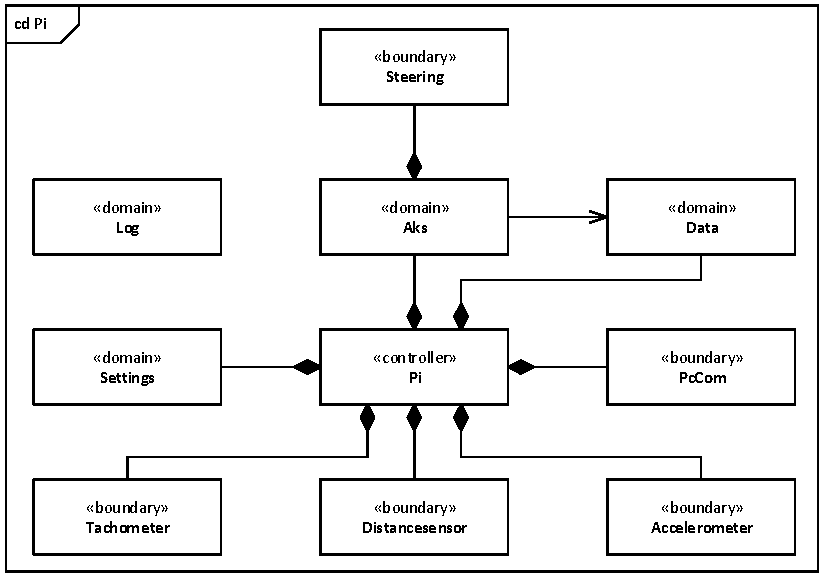
\includegraphics[width=\textwidth* 9/10]{../fig/diagrammer/bil/cd_pi.pdf}
\caption{Klasse diagram over Pi}
\label{fig:cd_pi}
\end{figure}

\subsubsection{Controller-klasse: Pi}
Controller-klassen Pi indeholder main funktionen og har derfor ansvaret for at styre slagets gang. Klassen skal derfor iværksætte initialisering af alle de klasser som den har ejerskab over. En af klassen ansvarsområder er at indsamle data fra sensorerne, og dette gøres ved at starte en særskilt tråd til dette. Denne tråd skal også sørge for at iværksætte Aks-klassen hver gang nye data er indsamlet.

\subsubsection{Domain-klasse: Aks}
Domain-klassen analyserer indkomne sensordata og i tilfælde at bilen er ved at køre ind i en forhindring, blokeres brugerinput og der styres udenom eller bremses.

\subsubsection{Domain-klasse: Data}
Denne klasse har til formål at indsamle alle sensordata i en datastruktur. Disse data gemmes i memory kan ikke overstige en defineret størrelse. Brugerinput gemmes ikke i denne klasse.

\subsubsection{Domain-klasse: Log}
Denne klasse har til formål at gemme samtlige systemhændelser i den fil, så kilden til eventuelle programcrash kan identificeres. Alle klasser på Pi har en reference til denne log, så de hver i sær kan skrive til den. På figur \ref{fig:cd_pi} er der undladt at lave pile fra alle klasser til denne, da dette vil gøre diagrammet uoverskueligt. 

\subsubsection{Domain-klasse: Settings}
Settings er datastruktur der indeholder indstillinger for maksimal hastighed, AKS status, og styretøjs kalibrering. Indstillingerne er gemt i en fil som kan tilgås af Pi-klassen og Steering-klassen.

\subsubsection{Boundary-klasse: PcCom}
Boundary-klassen PcCom håndterer kommunikationen imellem PC og Bil. Denne kommunikation sker vha. UDP via Wi-Fi.

\subsubsection{Boundary-klasse: Steering}
I denne klasse styres bilens aktautorer. Dette er altså en driver til både motoren der skaber fremdrift og servo-motoren der styrer forhjulene. Klassen tager ligeledes højde for brugers indstillinger.

\subsubsection{Boundary-klasse: Tachometer}
Denne klasse håndterer kommunikationen til bilens tachometer og konverterer sensordata til brugbar hastighedsmåling.

\subsubsection{Boundary-klasse: DistanceSensor}
Denne klasse håndterer kommunikationen til bilens afstandssensorer og konverterer sensordata til brugbar distancemålinger. Klassen håndterer alle fire sensorer.

\subsubsection{Boundary-klasse: Accelerometer}
Denne klasse håndterer kommunikationen til bilens accelerometer og konverterer sensordata til brugbar g-måling.

\clearpage

\subsection{Sekvensdiagrammer}
Herunder er udarbejdet sekvensdiagrammer for den funktionalitet som Pi blokken på bilen skal have. Der er tage udgangspunkt i de de tidligere fremstillede use cases. Sekvensdiagrammer for UC8 og UC12 er udeladt, da disse kun indeholder handlinger over interaktion imellem bruger og PC.

\begin{figure}[h]
\centering
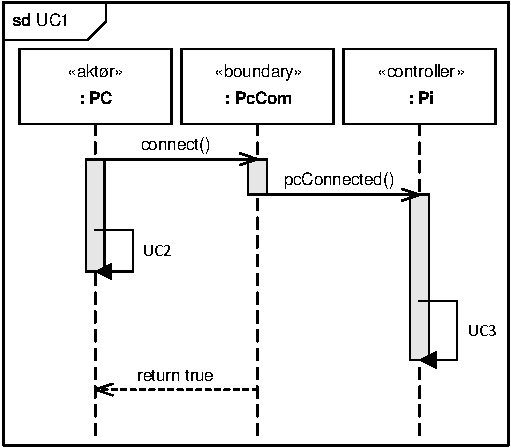
\includegraphics[]{../fig/diagrammer/bil/sd_uc1.pdf}
\caption{Sekvensdiagram over  bilens funktionalitet i UC1: Aktiver system}
\label{fig:sd_uc1_bil}
\end{figure}

\begin{figure}[h]
\centering
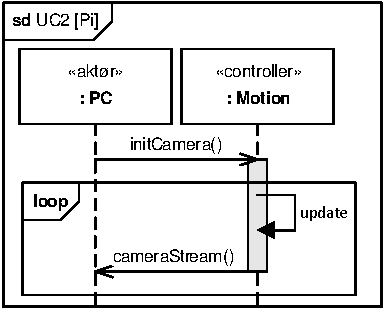
\includegraphics[]{../fig/diagrammer/bil/sd_uc2.pdf}
\caption{Sekvensdiagram over  bilens funktionalitet i UC2: Stream video}
\label{fig:sd_uc2_bil}
\end{figure}

\begin{landscape}

\begin{figure}[h]
\centering
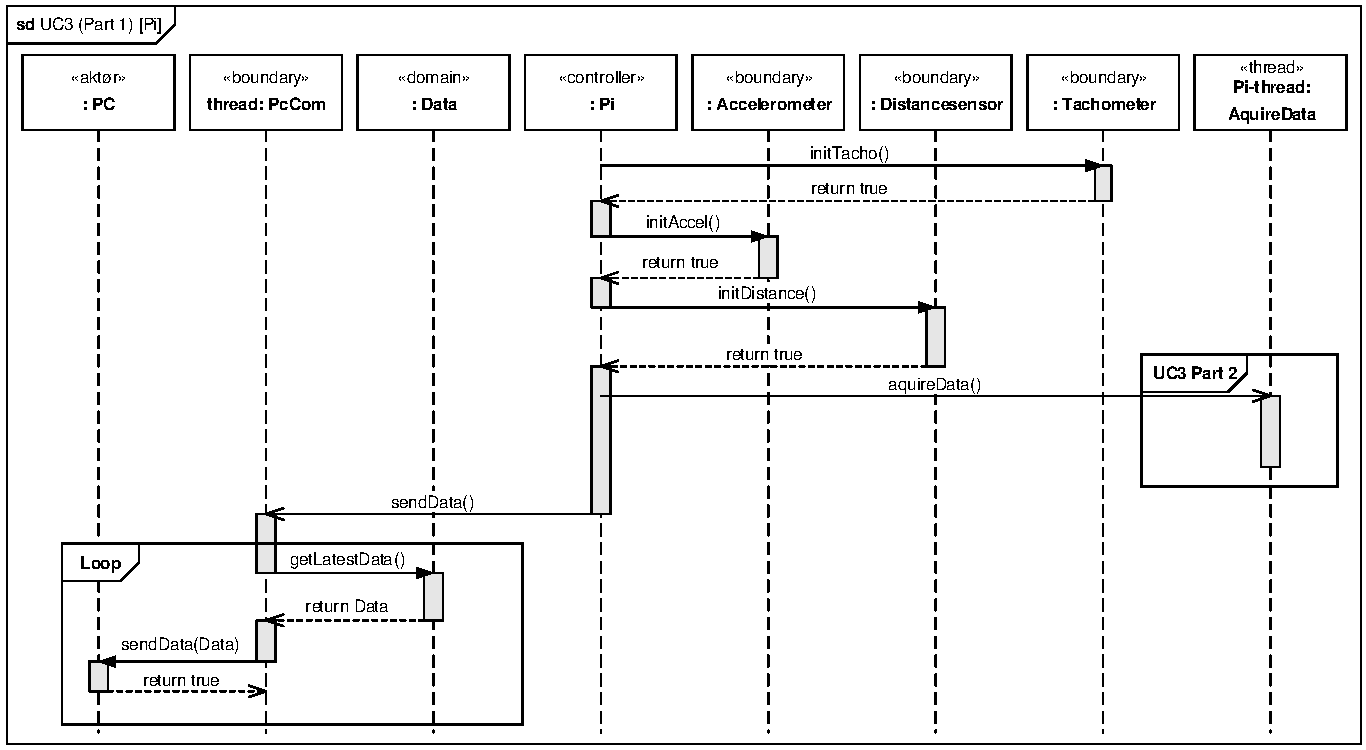
\includegraphics[]{../fig/diagrammer/bil/sd_uc3_1.pdf}
\caption{Sekvensdiagram over  bilens funktionalitet i UC3: Overvåg sensorer - Del 1}
\label{fig:sd_uc3_1_bil}
\end{figure}

\begin{figure}[h]
\centering
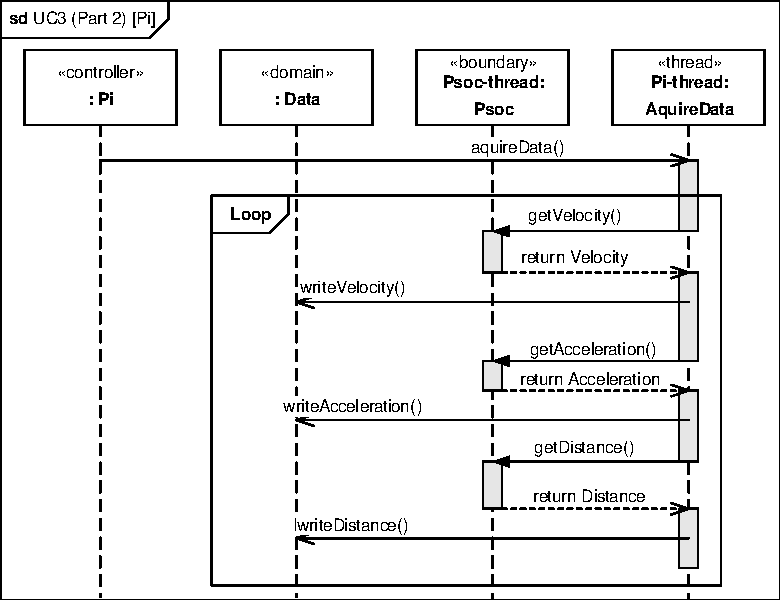
\includegraphics[]{../fig/diagrammer/bil/sd_uc3_2.pdf}
\caption{Sekvensdiagram over  bilens funktionalitet i UC3: Overvåg sensorer - Del 2}
\label{fig:sd_uc3_2_bil}
\end{figure}

\end{landscape}

\begin{figure}[h]
\centering
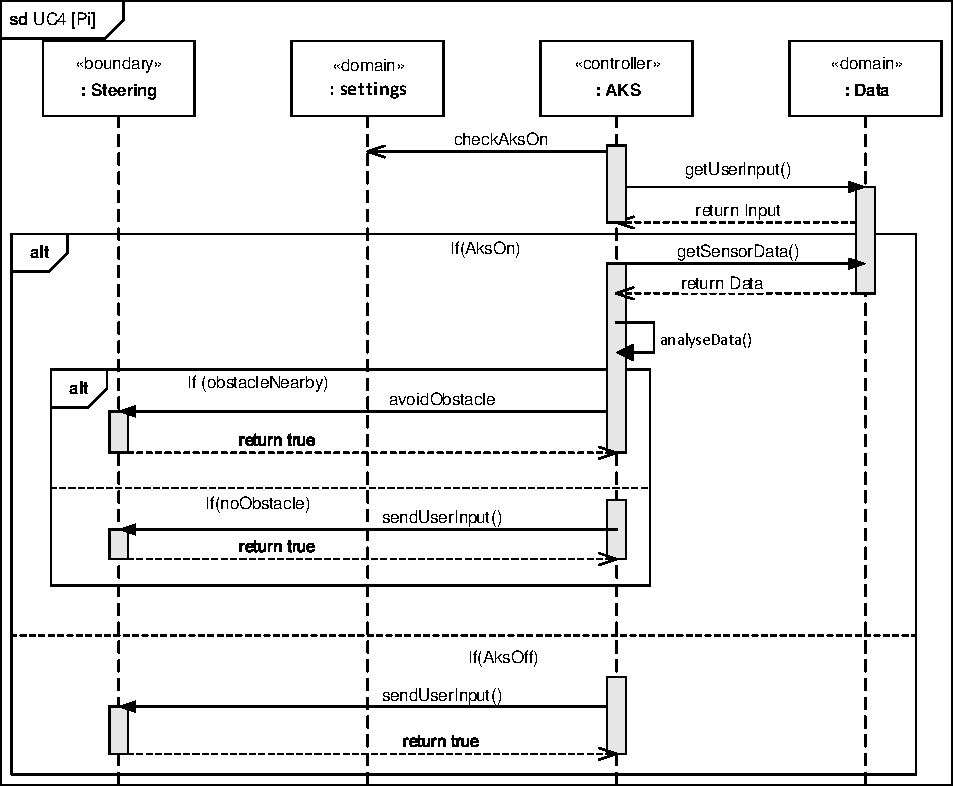
\includegraphics[]{../fig/diagrammer/bil/sd_uc4.pdf}
\caption{Sekvensdiagram over  bilens funktionalitet i UC4: Undvig forhindring}
\label{fig:sd_uc4_bil}
\end{figure}

\begin{figure}[h]
\centering
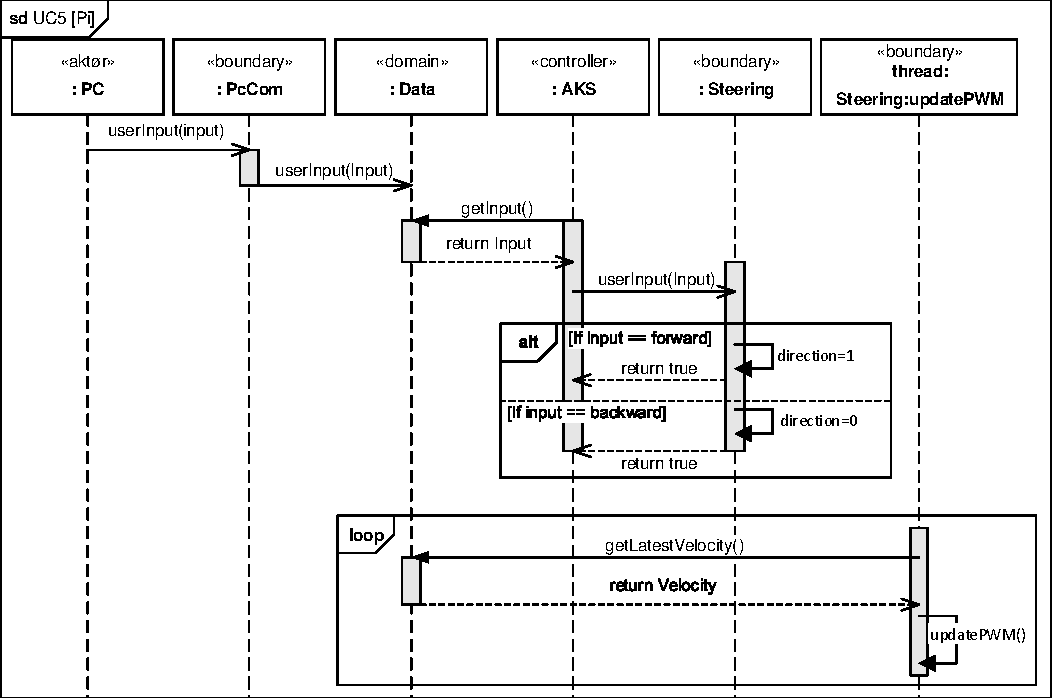
\includegraphics[]{../fig/diagrammer/bil/sd_uc5.pdf}
\caption{Sekvensdiagram over  bilens funktionalitet i UC5: Kør bil frem/tilbage}
\label{fig:sd_uc5_bil}
\end{figure}

\begin{figure}[h]
\centering
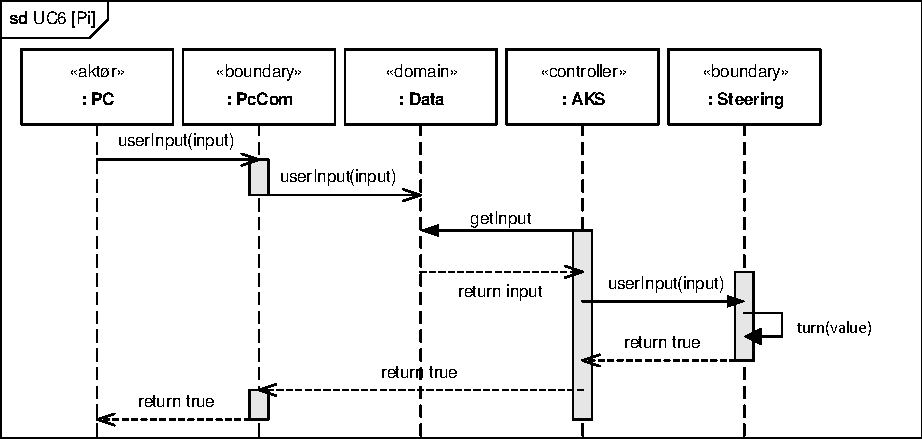
\includegraphics[]{../fig/diagrammer/bil/sd_uc6.pdf}
\caption{Sekvensdiagram over  bilens funktionalitet i UC6: Drej til højre/venstre}
\label{fig:sd_uc6_bil}
\end{figure}

\begin{figure}[h]
\centering
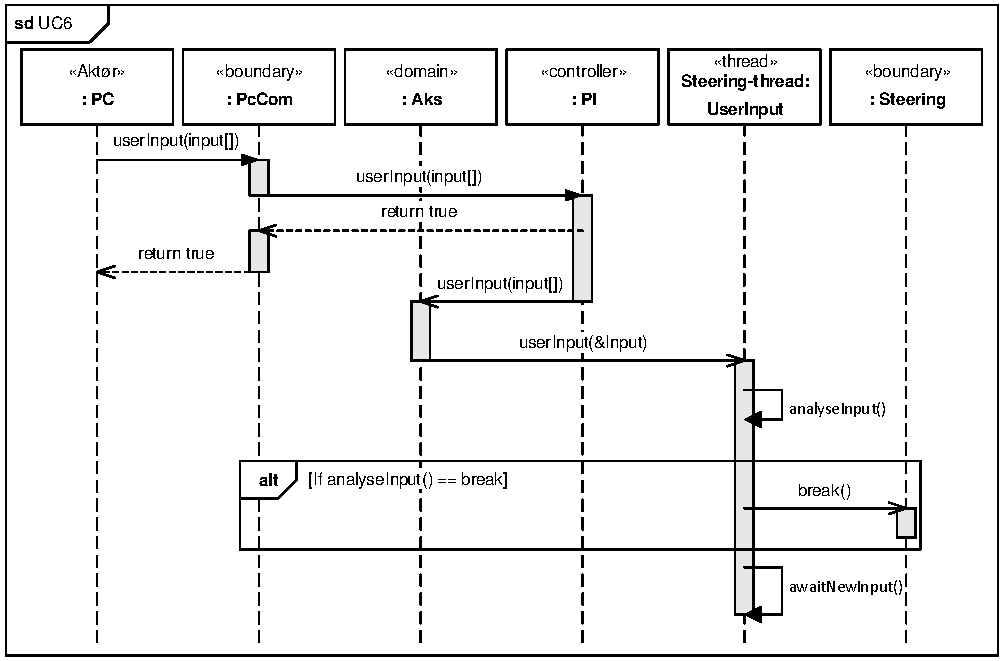
\includegraphics[]{../fig/diagrammer/bil/sd_uc7.pdf}
\caption{Sekvensdiagram over  bilens funktionalitet i UC7: Brems bil}
\label{fig:sd_uc7_bil}
\end{figure}

\begin{figure}[h]
\centering
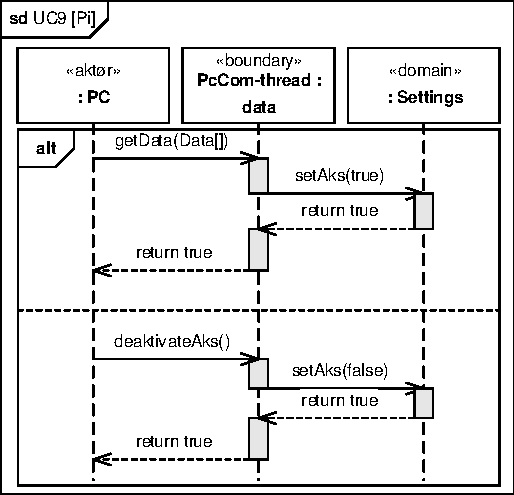
\includegraphics[]{../fig/diagrammer/bil/sd_uc9.pdf}
\caption{Sekvensdiagram over  bilens funktionalitet i UC9: Tænd/sluk AKS}
\label{fig:sd_uc9_bil}
\end{figure}

\begin{figure}[h]
\centering
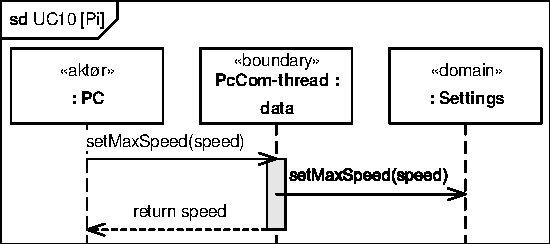
\includegraphics[]{../fig/diagrammer/bil/sd_uc10.pdf}
\caption{Sekvensdiagram over  bilens funktionalitet i UC10: Indstil makshastighed}
\label{fig:sd_uc10_bil}
\end{figure}

\begin{figure}[h]
\centering
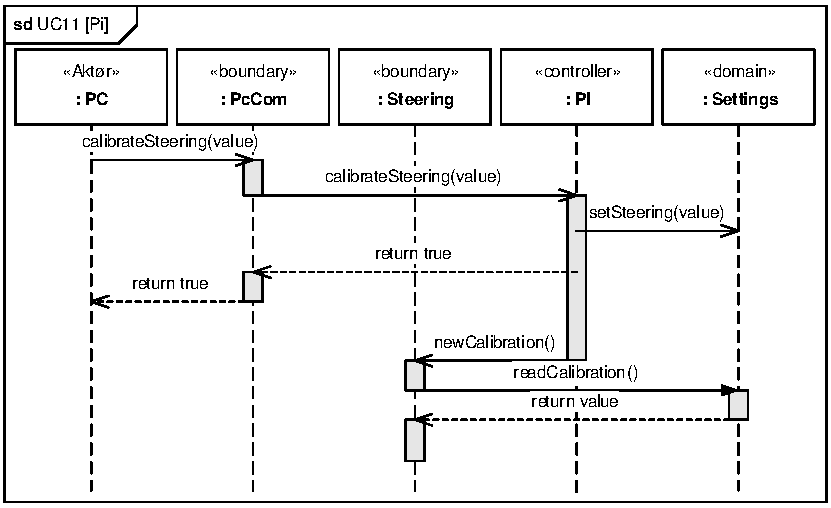
\includegraphics[]{../fig/diagrammer/bil/sd_uc11.pdf}
\caption{Sekvensdiagram over  bilens funktionalitet i UC11: Kalibrer styretøj}
\label{fig:sd_uc11_bil}
\end{figure}

\clearpage
\subsection{Klassebeskrivelser}
% ++++++++++++ Controller PSoC Master klassen ++++++++++++++
\subsubsection{Boundary-klasse: DistanceSensor}

\begin{figure}[h]
\centering
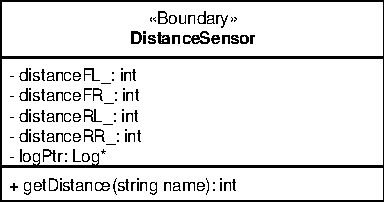
\includegraphics[]{../fig/diagrammer/bil/cd_distancesensor.pdf}
\caption{Klassebeskrivelse af boundary-klassen DistanceSensor}
\label{fig:cd_distancesensor}
\end{figure}

\textbf{Attributter}

\begin{table}[h]
\begin{tabularx}{\textwidth}{| Z | Z | L{10cm} |} \hline
Navn & Type & Beskrivelse \\\hline
\texttt{addrFL} & \texttt{int} &Adresse til forreste venstre afstandssensor.\\\hline
\texttt{addrFR} & \texttt{int} &Adresse til forreste højre afstandssensor.\\\hline
\texttt{addrRL} & \texttt{int} &Adresse til bagerste venstre afstandssensor.\\\hline
\texttt{addrRR} & \texttt{int} &Adresse til bagerste højre afstandssensor.\\\hline
\texttt{distanceFL} & \texttt{int} &Midlertidig variabel der indeholder afstanden fra forreste venstre afstandssensor.\\\hline
\texttt{distanceFR} & \texttt{int} &Midlertidig variabel der indeholder afstanden fra forreste højre afstandssensor.\\\hline
\texttt{distanceRL} & \texttt{int} &Midlertidig variabel der indeholder afstanden fra bagerste venstre afstandssensor.\\\hline
\texttt{distanceRR} & \texttt{int} &Midlertidig variabel der indeholder afstanden fra bagerste højre afstandssensor.\\\hline
\texttt{fd} & \texttt{int} &Variabel der anvendes som reference til i2c-bussen som sensorerne er tilkoblet\\\hline
\texttt{logEntry} & \texttt{string} &Variabel der indeholder reference til loggen.\\\hline
\end{tabularx}
\caption{Attributter for klassen DistanceSensor}
\label{table:attr_distancesensor}
\end{table}

\textbf{Metoder}

\begin{table}[h]
\begin{tabularx}{\textwidth}{| L{2.5 cm} | Z |} \hline
Prototype & \texttt{int getDistance(string name)} \\\hline
Parametre & \texttt{name} \newline Navnet på den sensor som der skal læses fra. Kan en af fire muligheder "FL", "FR", "RL" og "RR". \\\hline
Returværdi &  \texttt{int} \newline Afstanden for til nærmeste sensor for den pågældende sensor. Tallet er angivet i cm. \\\hline
Beskrivelse & Metoden læser afstanden som en afstandssensor befinder sig fra en forhindring. \\\hline
\end{tabularx}
\caption{Metodebeskrivelse for \texttt{getDistance}}
\label{table:met_getdistance}
\end{table}
\clearpage


Afstandssensorene leveres formonteret på chip hvor benene fra IC'en er trukket til harwinpins som let kan tilgås. Til kommunikationen benyttes følgende linjer: 

\begin{itemize}
	\item pin 7: VCC: Forsyning
	\item pin 6: GND: Reference
	\item pin 5: SCL: Clock
	\item pin 4: SDA: Data
	\item pin 3: Benyttes ikke
	\item pin 2: Status
	\item pin 1: Temp adresse 
\end{itemize}

Data kommunikeres på SDA-linjen med reference til clock'en. ''Status'' benyttes til at angive om sensoren er i gang med at performe en ''range reading''. 
Pin'en holdes højt så længe sensoren scanner, og trækkes lavt når operationen er fuldført og data kan leveres. Når pin'en er høj ignoreres al I2C-kommunikation.

For at initiere sensoren, ''Temp-adresse''-pin'en hvor der sendes en unik 7-bit adresse til sensoren.
   
Afstandssensorene benytter sig af I2C-bussen til kommunikation med Pi'en. Hertil benyttes I2C-tools biblioteket.
Dette bibliotek skal derfor hentes og aktiveres i linux-distrubutionen.

I2C device filer er CDD med major-nummer 89, og hver enkelt adaptor der er tilkoblet systemet får vedhæftet et minor-nummer, 
disse device filer findes i /dev/i2c-X, hvor X er et unik minor-nummer fra 0-256. Herfter er hver enkelt i2c-adaptor nu identificerbar og kan tilgås enkeltvis. 

Herefter skrives en klasse der kan håndtere de ønskede kald til de 4 afstandssensorer. 
I dette tilfælde ønskes der at implementere initDistance() og en getDistance() og i disse funktioner benyttes systemkald til at tilgå Hardwaren direkte, og aflæse de 4 sensorer via I2C-bussen.
\clearpage
% ++++++++++++ Controller PSoC Master klassen ++++++++++++++
\subsubsection{Domain-klasse: Data}

\begin{figure}[h]
\centering
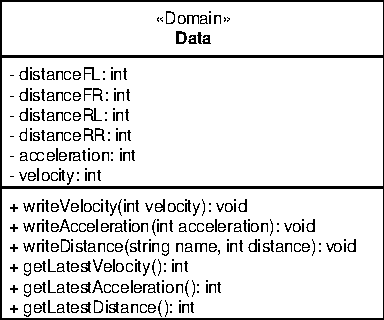
\includegraphics[]{../fig/diagrammer/bil/cd_data.pdf}
\caption{Klassebeskrivelse for domain-klassen Data}
\label{fig:cd_data}
\end{figure}

\textbf{Attributter}

\begin{table}[h]
\begin{tabularx}{\textwidth}{| Z | Z | L{10cm} |} \hline
Navn & Type & Beskrivelse \\\hline
\texttt{distanceFL} & \texttt{int} &Variabel der indeholder afstanden til en evt. forhindring ved forreste venstre hjørne af bilen i cm.\\\hline
\texttt{distanceFR} & \texttt{int} &Variabel der indeholder afstanden til en evt. forhindring ved forreste højre hjørne af bilen i cm.\\\hline
\texttt{distanceRL} & \texttt{int} &Variabel der indeholder afstanden til en evt. forhindring ved bageste venstre hjørne af bilen i cm.\\\hline
\texttt{distanceRR} & \texttt{int} &Variabel der indeholder afstanden til en evt. forhindring ved bageste højre hjørne af bilen i cm.\\\hline
\texttt{acceleration} & \texttt{int} &Variabel der indeholder bilens aktuelle acceleration i G.\\\hline
\texttt{velocity} & \texttt{int} &Variabel der indeholder bilens aktuelle hastighed i km/t.\\\hline
\end{tabularx}
\caption{Attributter for klassen Data}
\label{table:attr_data}
\end{table}
%TODO ret enheder

\textbf{Metoder}

\begin{table}[h]
\begin{tabularx}{\textwidth}{| L{2.5 cm} | Z |} \hline
Prototype & \texttt{void writeVelocity(int velocity)} \\\hline
Parametre & \texttt{velocity} \newline Den hastighed der skal indlæses. \\\hline
Returværdi &  \texttt{void} \newline \\\hline
Beskrivelse & Metoden indlæser den nyeste værdi af hastigheden i datastrukturen. \\\hline
\end{tabularx}
\caption{Metodebeskrivelse for \texttt{writeVelocity}}
\label{table:met_writeVelocity}
\end{table}

\begin{table}[h]
\begin{tabularx}{\textwidth}{| L{2.5 cm} | Z |} \hline
Prototype & \texttt{void writeAcceleration(int acceleration)} \\\hline
Parametre & \texttt{acceleration} \newline Den acceleration der skal indlæses. \\\hline
Returværdi &  \texttt{void} \newline \\\hline
Beskrivelse & Metoden indlæser den nyeste værdi af accelerationen i datastrukturen. \\\hline
\end{tabularx}
\caption{Metodebeskrivelse for \texttt{writeAcceleration}}
\label{table:met_writeAcceleration}
\end{table}

\begin{table}[h]
\begin{tabularx}{\textwidth}{| L{2.5 cm} | Z |} \hline
Prototype & \texttt{void  writeDistance(string name, int distance)} \\\hline
Parametre & \texttt{name} \newline Navnet på den sensor som der skal indlæses data fra. Kan være FL, FR, RL eller RR. \newline \newline
			\texttt{distance} \newline
			Afstanden der fra den pågældende sensor der skal indlæses i datastrukturen.\\\hline
Returværdi &  \texttt{void} \newline \\\hline
Beskrivelse & Metoden indlæser den nyeste værdi af fra en vilkårlig afstandssensor i datastrukturen. \\\hline
\end{tabularx}
\caption{Metodebeskrivelse for \texttt{writeDistance}}
\label{table:met_writeDistance}
\end{table}

\begin{table}[h]
\begin{tabularx}{\textwidth}{| L{2.5 cm} | Z |} \hline
Prototype & \texttt{int getLatestVelocity()} \\\hline
Parametre &  ~\newline \\\hline
Returværdi &  \texttt{int} \newline Den nyeste hastighedsmåling. \\\hline
Beskrivelse & Metoden returnerer den nyeste hastighedsmåling der er indlæst i datastrukturen. \\\hline
\end{tabularx}
\caption{Metodebeskrivelse for \texttt{getLatestVelocity}}
\label{table:met_getLatestVelocity}
\end{table}

\begin{table}[h]
\begin{tabularx}{\textwidth}{| L{2.5 cm} | Z |} \hline
Prototype & \texttt{int getLatestAcceleration()} \\\hline
Parametre &  ~\newline \\\hline
Returværdi &  \texttt{int} \newline Den nyeste accelerationsmåling. \\\hline
Beskrivelse & Metoden returnerer den nyeste accelerationsmåling der er indlæst i datastrukturen. \\\hline
\end{tabularx}
\caption{Metodebeskrivelse for \texttt{getLatestAcceleration}}
\label{table:met_getLatestAcceleration}
\end{table}

\begin{table}[h]
\begin{tabularx}{\textwidth}{| L{2.5 cm} | Z |} \hline
Prototype & \texttt{int getLatestDistance(string name)} \\\hline
Parametre &  \texttt{name}\newline Navnet på den sensor som der ønskes data fra. Kan være FL, FR, RL eller RR.\\\hline
Returværdi &  \texttt{int} \newline Den nyeste afstandsmåling fra den angivne sensor. \\\hline
Beskrivelse & Metoden returnerer den nyeste afstandsmåling fra den angivne sensor. \\\hline
\end{tabularx}
\caption{Metodebeskrivelse for \texttt{getLatestDistance}}
\label{table:met_getLatestDistance}
\end{table}
\clearpage
% ++++++++++++ Domain Pi AKS klassen ++++++++++++++
\subsubsection{Domain-klasse: Aks}\label{sec:aks_design}

\begin{figure}[h]
\centering
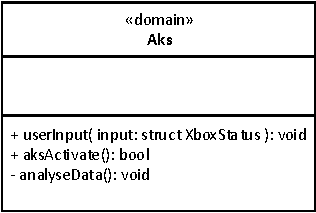
\includegraphics[scale=1]{../fig/diagrammer/bil/cd_aks.pdf}
\caption{Klassebeskrivelse for domain-klassen Aks}
\label{fig:cd_aks}
\end{figure}

\textbf{Attributter}

\begin{table}[h]
\begin{tabularx}{\textwidth}{| Z | Z | L{9cm} |} \hline
Navn & Type & Beskrivelse \\\hline
\texttt{MySteering} & \texttt{Steering} & Styretøjsklassen, bruges når Aks skal påvirke bilens hastighed eller retning.\\\hline
\texttt{MyData} & \texttt{Data*} & Pointer til bilens datastruktur.\\\hline
\texttt{MySettings} & \texttt{Settings*} & Pointer til Settingsklassen. \\\hline
\texttt{MyLog} & \texttt{Log*} & Pointer til loggen. \\\hline
\texttt{state} & \texttt{aksStates} & Husker hvilket stadie bilen er i, kan skifte mellem at stå stille, køre fremad/bagud eller trille. \\\hline
\texttt{proxSensors} & \texttt{int*} & Et array med nuværende værdier fra afstandssensorer \\\hline
\texttt{old\_proxSensors} & \texttt{int*} & Et array der holder de foregående værdier fra afstandssensorer \\\hline
\texttt{latestUserInput} & \texttt{UserInput} & Gemmer de seneste input fra brugeren. \\ \hline
\end{tabularx}
\caption{Attributter for klassen Aks}
\label{table:attr_aks}
\end{table}

\textbf{Metoder}


%----------------- aksActivate -------------------
\begin{table}[h]
\begin{tabularx}{\textwidth}{| L{2.5 cm} | Z |} \hline
Prototype & \texttt{void aksActivate(void)} \\\hline
Parametre & \texttt{void}  \\\hline
Returværdi &  \texttt{bool} \newline Returnerer \texttt{TRUE} hvis det gik godt og \texttt{FALSE} hvis der skete fejl undervejs. \\\hline
Beskrivelse & Metoden kaldes når det automatiske anti-kollisionssystem skal aktiveres. Forhindrer samtidigt input fra brugeren kortvarigt. \\\hline
\end{tabularx}
\caption{Metodebeskrivelse for \texttt{aksActivate}}
\label{table:met_aks_aksActivate}
\end{table}

%----------------- analyseData -------------------
\begin{table}[h]
\begin{tabularx}{\textwidth}{| L{2.5 cm} | Z |} \hline
Prototype & \texttt{void analyseData(void)} \\\hline
Parametre & \texttt{void}  \\\hline
Returværdi &  \texttt{void}  \\\hline
Beskrivelse & Metoden analyserer indhentet data fra Data klassen og vurderer hvilken type af undvigelse der bedst passer. Aktiverer herefter Steering-klassen for at bilen skal undvige forhindringen. \\\hline
\end{tabularx}
\caption{Metodebeskrivelse for \texttt{analyseData}}
\label{table:met_aks_analyseData}
\end{table}
\clearpage
\subsubsection{Boundry-klasse: PcCom}

\begin{figure}[h]
\centering
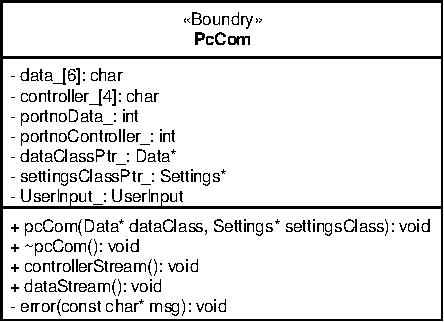
\includegraphics[]{../fig/diagrammer/bil/cd_pccom.pdf}
\caption{Klassebeskrivelse for boundry-klassen PcCom}
\label{fig:cd_pccom}
\end{figure}

\textbf{Attributter}

\begin{table}[h]
\begin{tabularx}{\textwidth}{| Z | Z | L{10cm} |} \hline
Navn & Type & Beskrivelse \\\hline
\texttt{data\_}					& \texttt{char[6]}	&Array af typen char med variable der indeholder hhv. maksimal hastighed, nuværende hastighed, afstand til nærmeste forhindring, nuværende acceleration, AKS status og styretøjs calibrering.\\\hline

\texttt{controller\_}			& \texttt{char[4]}	&Array af typen char med variable der indeholder bruger input for hhv. frem, tilbage, drej og stop.\\\hline

\texttt{portnoData\_}			& \texttt{int}		&Variabel der indeholder portnummeret til den TCP socket der har med overførelse til og fra data\_ array'et.\\\hline

\texttt{portno- Controller\_}	& \texttt{int}		&Variabel der indeholder portnummeret til den TCP socket der har med overførelse til og fra controller\_ array'et.\\\hline

\texttt{dataClassPtr\_}			& \texttt{Data*}	&En pointer til det objekt af typen Data der ønskes læst og skrevet data til.\\\hline

\texttt{settings- ClassPtr\_}	& \texttt{Settings*}&En pointer til det objekt af typen Settings der ønskes skrevet data til.\\\hline

\texttt{UserInput\_}			& \texttt{UserInput}&En struct af typen UserInput der har fire chars, hhv. frem, tilbage, drej og stop.\\\hline
\end{tabularx}
\caption{Attributter for klassen PcCom}
\label{table:attr_pccom}
\end{table}

\clearpage

\textbf{Metoder}

\begin{table}[h]
\begin{tabularx}{\textwidth}{| L{2.5 cm} | Z |} \hline
Prototype 	& \texttt{void PcCom(Data* dataClass, Settings* settingsClass, Log* logClass)} \\\hline
Parametre 	& \texttt{dataClass} 		\newline Det objekt af typen Data der ønskes bearbjedet af PcCom. \newline \newline
			  \texttt{settingsClass} 	\newline Det objekt af typen Settings der ønskes bearbjedet af PcCom. \newline \newline
			  \texttt{logClass}	 		\newline Det objekt af typen Log der ønskes skrevet til af PcCom. \\\hline
Returværdi	& \texttt{void} 			\newline \\\hline
Beskrivelse	& Constructor til klassen PcCom. \newline \\\hline
\end{tabularx}
\caption{Metodebeskrivelse for constructoren af \texttt{PcCom} klassen}
\label{table:met_pccom}
\end{table}

\begin{table}[h]
\begin{tabularx}{\textwidth}{| L{2.5 cm} | Z |} \hline
Prototype 	& \texttt{void $\sim$PcCom()} \\\hline
Parametre 	& \texttt{void}				\newline \\\hline
Returværdi	& \texttt{void} 			\newline \\\hline
Beskrivelse	& Destructor til klassen PcCom. \newline \\\hline
\end{tabularx}
\caption{Metodebeskrivelse for destructoren af \texttt{PcCom} klassen}
\label{table:met_pccom_de}
\end{table}

\begin{table}[h]
\begin{tabularx}{\textwidth}{| L{2.5 cm} | Z |} \hline
Prototype 	& \texttt{void controllerStream()} \\\hline
Parametre 	& \texttt{void}				\newline \\\hline
Returværdi	& \texttt{void} 			\newline \\\hline
Beskrivelse	& Denne funktion har til formål at initialisere og køre en TCP server. Denne server skal streame hhv. frem-, tilbage-, drej- og stop-kommandoer fra PC'en til bilen. Herefter skal den sende den streamede data til Data klassen. \\\hline
\end{tabularx}
\caption{Metodebeskrivelse for \texttt{controllerStream()}}
\label{table:met_controllerstream}
\end{table}

\clearpage

\begin{table}[h]
\begin{tabularx}{\textwidth}{| L{2.5 cm} | Z |} \hline
Prototype 	& \texttt{void dataStream()} \\\hline
Parametre 	& \texttt{void}				\newline \\\hline
Returværdi	& \texttt{void} 			\newline \\\hline
Beskrivelse	& Denne funktion har til formål at initialisere og køre en TCP server. Denne server skal streame hhv. maksimal hastighed, nuværende hastighed, afstand til nærmeste forhindring, nuværende acceleration, AKS status og styretøjs calibrering fra PC'en til bilen. Herefter skal den sende den streamede data til Data og Settings klassen. \\\hline
\end{tabularx}
\caption{Metodebeskrivelse for \texttt{dataStream()}}
\label{table:met_datastream}
\end{table}

\begin{table}[h]
\begin{tabularx}{\textwidth}{| L{2.5 cm} | Z |} \hline
Prototype 	& \texttt{void error(string msg)} \\\hline
Parametre 	& \texttt{msg}				\newline En pågældende fejl-besked i form af en string. \\\hline
Returværdi	& \texttt{void} 			\newline \\\hline
Beskrivelse	& Denne funktion har til formål at skrive en fejl til log, hvis der opstår en fejl. \newline \\\hline
\end{tabularx}
\caption{Metodebeskrivelse for \texttt{error()}}
\label{table:met_error}
\end{table}